% Paper 2 — citation-network analysis of Saudi legislation.
% Target: Artificial Intelligence and Law (Springer).
%
% Uses Springer's sn-jnl class when present (Overleaf's Springer Nature
% template, or the class dropped next to this file); otherwise a
% self-contained single-column fallback compiles on a plain TeX Live.
\IfFileExists{sn-jnl.cls}{%
  \documentclass[sn-basic]{sn-jnl}%
  \newcommand{\usingsnstyle}{}%
}{%
  \documentclass[11pt]{article}%
  \usepackage[a4paper,top=2.5cm,bottom=2.5cm,left=3cm,right=3cm]{geometry}%
  \usepackage{times}%
  \usepackage[round]{natbib}%
  \usepackage{setspace}%
  \onehalfspacing%
  \usepackage[hidelinks]{hyperref}%
}

\usepackage[T1]{fontenc}
\usepackage[utf8]{inputenc}
\usepackage{microtype}
\usepackage{booktabs}
\usepackage{graphicx}
\usepackage{url}
\emergencystretch=3em

\title{Vertical Elaboration or Horizontal Integration? A Citation-Network
Analysis of Saudi Arabian Legislation}

\ifdefined\usingsnstyle
  \author*[1]{\fnm{Abdullah} \sur{Almohammedi}}\email{abdullah.m.almohammedi@gmail.com}
  \affil[1]{\orgname{Independent Researcher}}
\else
  \author{Abdullah Almohammedi \\
    Independent Researcher \\
    \texttt{abdullah.m.almohammedi@gmail.com} \\
    ORCID: \href{https://orcid.org/0009-0001-0832-0995}{0009-0001-0832-0995}}
  \date{}
\fi

\begin{document}

\maketitle

\begin{abstract}
Network analysis of legal citation has produced a substantial literature for
the United States and Europe, but the legal systems of the Arab world have
remained outside it, for want of machine-readable statutory corpora. Using a
newly released, provenance-annotated corpus of Saudi Arabian legislation, we
construct and analyse what is, to our knowledge, the first citation
network over Saudi statutory law:
290 legislative instruments, 15{,}689 articles, and 585 extracted
inter-instrument references. We first address a problem that the citation
literature typically leaves implicit: the extractor that resolves a cited law
name to a target instrument is itself fallible. Validating every resolved
edge against the target's registered title and adjudicating the residue by
hand, we find a 3.3\% misresolution rate and analyse only the 410 surviving
citations. We then separate \emph{vertical} citations, in which a subordinate
instrument elaborates its own parent statute, from \emph{horizontal}
citations that cross instrument families. The distinction is not cosmetic:
the Labour Law appears to rival the Companies Law as the system's leading hub
until its eight annexes are recognised as part of its own family, after which
its horizontal citation count falls by more than a third and the Companies
Law stands alone. Horizontal citations nevertheless account for 70.5--74.4\%
of the network depending on how family boundaries are drawn, so Saudi
legislation is genuinely cross-referential rather than merely hierarchical.
The horizontal network is sparse (164 instruments, 206 edges) and highly
concentrated: ten instruments receive 58\% of all horizontal citations, led
by the Companies Law (46 citations from 26 distinct instruments). Breadth and
depth diverge sharply --- the Capital Market Law draws 26 citations from only
9 instruments, while the Criminal Procedure Law draws 13 from 13 --- a
contrast that raw citation counts conceal. Cross-referencing the citation
network against a hand-classified supersession graph, we identify live
instruments that still cite repealed predecessors, and we map the instruments
that Saudi legislation cites but that no consolidated machine-readable source
yet covers. We discuss what these structures imply for legal informatics,
retrieval-augmented legal AI, and legislative maintenance.
\end{abstract}

\ifdefined\usingsnstyle
\keywords{Legal citation networks, Saudi Arabia, Legislation, Legal
informatics, Network analysis, Legal data quality}
\else
\vspace{1em}\noindent\textbf{Keywords:} Legal citation networks $\cdot$ Saudi
Arabia $\cdot$ Legislation $\cdot$ Legal informatics $\cdot$ Network analysis
$\cdot$ Legal data quality
\vspace{1em}
\fi

\section{Introduction}
\label{sec:intro}

A legal system is not a list of laws. Statutes refer to one another:
they borrow definitions, defer to procedures, carve out exceptions, and
assign jurisdiction. Those references form a network, and for two decades
that network has been an object of quantitative study --- initially for
judicial precedent \citep{fowler2007network}, then for statutory corpora
\citep{katz2014complexity, coupette2021measuring}. The results have been
substantive rather than decorative: they identify which instruments carry
structural load, how complexity accumulates, and how legal systems change
over time.

That literature is almost entirely Anglo-American and European. The legal
systems of the Arab world are absent from it, and the reason is prosaic
rather than intellectual: the analysis requires a machine-readable statutory
corpus with resolvable citations, and for those jurisdictions no such
resource has been available. Saudi Arabia is a case in point. Its
legislation is published officially in the \emph{Umm Al-Qura} gazette and on
government portals as human-readable documents; it has recently undergone a
major codification wave, including a Civil Transactions Law of 721 articles,
a new Companies Law, a new Evidence Law, and a new Personal Status Law; and
nothing about its citation structure has been measured.

This paper reports what is, to our knowledge, the first such measurement. It
uses a recently released
corpus of Saudi legislation --- 290 instruments and 15{,}689 article-level
records with per-record provenance \citep{almohammedi2026corpus} --- and the
citation graph derived from it, and asks three questions.

\emph{Is the network hierarchical or integrated?} Saudi legislation, like
most civil-law systems, is organised in families: a statute and the
implementing regulation that elaborates it. If most citations simply run
from a regulation to its own parent, the network is an artefact of drafting
hierarchy and says little about systemic integration. We therefore separate
vertical from horizontal citation and analyse them apart
(Section~\ref{sec:vh}). They behave differently, and the separation changes
which instruments count as central.

\emph{Which instruments carry structural load?} We report centrality over
the validated horizontal network and distinguish instruments cited by many
others from instruments cited often by few (Section~\ref{sec:hubs}).

\emph{Does the network contain maintenance defects?} Cross-referencing the
citation graph against a hand-classified supersession graph, we look for
live instruments that still cite repealed predecessors
(Section~\ref{sec:dangling}), and we map what Saudi legislation cites that
is not yet available in consolidated machine-readable form
(Section~\ref{sec:absent}).

A fourth contribution is methodological and cuts across the rest. Citation
extraction over statutory text involves two distinct steps --- detecting
that a citation occurred, and resolving the cited name to an instrument ---
and the second is fallible in ways that quietly corrupt network results. We
validate every resolved edge and report the error rate rather than assuming
it away (Section~\ref{sec:validation}). We recommend this as standard
practice for legal citation-network studies built on automatic extraction.

\section{Related work}
\label{sec:related}

\paragraph{Legal citation networks.}
\citet{fowler2007network} established the network-analytic study of legal
citation with an analysis of United States Supreme Court precedent, using
centrality to measure the legal importance of individual cases.
\citet{katz2014complexity} extended the approach from case law to statutory
law, treating the United States Code as a structured object whose complexity
can be measured. \citet{coupette2021measuring} generalised the framework to
legislation over time and across jurisdictions, comparing the statutory and
regulatory corpora of the United States and Germany. This paper follows that
statutory line rather than the precedential one: the unit of analysis is an
enacted instrument, and the edges are cross-references between instruments.

\paragraph{Legal corpora and standards.}
The machine-readable substrate for such work has grown considerably ---
Akoma Ntoso \citep{palmirani2011akoma} and the European Legislation
Identifier for structure, and large corpora such as the Pile of Law
\citep{henderson2022pileoflaw} and MultiLegalPile
\citep{niklaus2024multilegalpile} for text. None covers Saudi legislation,
and Arabic is at best marginal in them. The corpus used here
\citep{almohammedi2026corpus} was built specifically to close that gap; the
present paper is an analysis of the legal system it describes rather than a
description of the resource.

\paragraph{Citation extraction and its reliability.}
Work on legal citation extraction has generally reported detection
performance, while the downstream step --- resolving a detected citation to
the instrument it names --- receives less scrutiny in network studies that
consume its output. Where corpora are curated by hand this matters little.
Where edges are produced by automatic resolution, as here, misresolution
propagates directly into centrality rankings, and we treat it as a first-class
methodological concern (Section~\ref{sec:validation}).

\section{Data and method}
\label{sec:method}

\subsection{Corpus and citation graph}

The corpus comprises 290 Saudi legislative instruments --- 201 statutory
laws, 64 statutory regulations, 24 implementing regulations, and one set of
procedural rules --- structured into 15{,}689 article-level records with
per-record source provenance under a four-tier verification taxonomy
\citep{almohammedi2026corpus}. A deterministic extractor scans every record
for statutory citations and emits 3{,}607 references, of which 3{,}022 are
internal to a single instrument and 585 point from one instrument to
another. This paper analyses the 585 inter-instrument references; internal
cross-references describe the architecture of individual statutes rather
than the structure of the system.

Of the 585, the extractor resolves 424 to a specific instrument in the
corpus. The remaining 161 name an instrument the corpus does not contain;
they are excluded from the network but analysed separately in
Section~\ref{sec:absent}, where they turn out to be informative in their own
right.

\subsection{Edge validation}
\label{sec:validation}

Resolution errors are not hypothetical. The extractor matches a cited name
--- often truncated, inflected, or embedded in surrounding text --- against
the corpus's registered instrument titles, and some matches are simply
wrong. In one case a citation to the (uncodified) civil-service discipline
regime resolves to the Contractors Classification Law; in another, a
reference to the phrase ``Islamic Sharia'' resolves to the Public
Prosecution Law. Left in place, such edges add spurious in-degree to
arbitrary instruments.

We therefore validated every resolved edge before analysis. Each cited name
and the registered Arabic title of its resolved target were normalized
(diacritics and tatweel stripped, alef, teh-marbuta and alef-maqsura
variants folded) and reduced to content tokens by removing structural words
such as ``law'', ``regulation'', ``implementing'', ``previous'', and decree
formulae. An edge whose cited name shares at least one content token with
its target's title was accepted automatically; 408 of 424 edges cleared this
test. The remaining 16 were adjudicated by hand against the raw citation
text, and the decisions are published with the analysis code. Two proved
correct --- a morphological variant of ``bankruptcy'', and a truncation of
``valuers'' --- and 14 were misresolutions and were dropped.

The resulting misresolution rate among resolved edges is \textbf{3.3\%}
(14/424). Analysis proceeds on the surviving \textbf{410} citations. We
report this figure not as a criticism of the extractor, whose published
caveats already flag confidence levels, but because a network study that
consumes automatic resolution silently inherits its errors, and 3.3\% is
large enough to move a ranking of instruments whose citation counts differ
by one or two.

\subsection{Vertical and horizontal citation}
\label{sec:vh}

Saudi legislation is drafted in families: a statute is typically accompanied
by an implementing regulation, and sometimes by annexes, model forms, and
procedural rules. A regulation necessarily cites its own parent statute,
often repeatedly. Counting those citations alongside references that cross
from one body of law into another conflates two different phenomena.

Family membership must therefore be recovered before anything is counted,
and how it is recovered matters. Deriving families by stripping structural
suffixes from instrument identifiers is the obvious approach and it is
wrong: it splits the Labour Law's model contract forms and accessibility
arrangements from the Labour Law itself, and would classify 36 parent-child
citations as horizontal. We instead take family membership from the corpus's
own subject-matter grouping, which joins each statute with its regulation
and annexes --- the Labour Law family spans eight components --- and recover
it by mapping every track's data files to the grouping key its records
carry. A residual ambiguity remains where a subordinate instrument carries
its own grouping key derived from the parent's (bankruptcy fees under
bankruptcy), so we report both readings: a \emph{strict} one that treats such
keys as separate families and a \emph{prefix} one that merges them, giving
upper and lower bounds on the horizontal share.

The distinction is consequential in two directions. Instruments that appear
prominent on raw counts --- the Anti-Narcotics Law (15 citations) and the
Traffic Law (10) --- receive those citations from exactly one source each,
their own implementing regulation, and disappear from the horizontal ranking
entirely. More strikingly, the Labour Law falls from 36 horizontal citations
under the naive family definition to 23 under the corrected one, because
thirteen of its citations come from its own annexes. Under the naive
definition the Labour Law and the Companies Law look like twin hubs of
comparable weight; under the corrected one the Companies Law stands alone.
An analysis that skipped this step would have reported a headline finding
that the data do not support. Unless stated otherwise, the results below
concern the horizontal network under the prefix reading.

\section{Results}
\label{sec:results}

\subsection{Global structure}

\begin{table}[t]
\centering
\small
\begin{tabular}{lr}
\toprule
\textbf{Measure} & \textbf{Value} \\
\midrule
Instruments in the corpus (nodes) & 290 \\
Instruments with at least one citation & 201 \\
Distinct citing pairs (edges) & 257 \\
Citations carried & 410 \\
\midrule
Vertical citations, strict family reading & 105 \\
Vertical citations, prefix family reading & 121 \\
Horizontal citations (across families) & 289--305 \\
Horizontal share & 70.5--74.4\% \\
\midrule
Horizontal network: instruments & 164 \\
Horizontal network: edges & 206 \\
Share of horizontal citations to the top ten & 58.1\% \\
Density over the citing subgraph & 0.0064 \\
Weakly connected components & 12 \\
Largest component & 175 \\
Reciprocal instrument pairs & 2 \\
\bottomrule
\end{tabular}
\caption{Structure of the validated Saudi legislative citation network.}
\label{tab:structure}
\end{table}

Table~\ref{tab:structure} summarises the network. Three features stand out.

First, the network is \textbf{predominantly horizontal}: between 289 and 305
of 410 citations --- 70.5\% to 74.4\% depending on where family boundaries
are drawn --- cross instrument families. Saudi legislation is therefore
genuinely cross-referential; the citation structure is not an artefact of
statute-plus-regulation drafting. This is worth stating plainly because the
opposite result was entirely plausible \emph{a priori} for a codified
civil-law system with a strong statute/regulation hierarchy. It is equally
worth noting that a naive family definition inflates this figure to 79.3\%,
which is why we report the bounds rather than a single number.

Second, the network is \textbf{sparse but connected}. Density over the
citing subgraph is 0.0064, yet 175 of the 201 citing instruments fall into a
single weakly connected component. Saudi law is not a set of isolated
regimes: nearly every instrument that cites anything is, directly or
transitively, connected to nearly every other. The remaining 11 components
are small and topically isolated.

Third, citation is \textbf{almost entirely asymmetric}: only two pairs of
instruments cite each other. Legislative cross-reference in this corpus runs
one way, from later or subordinate instruments toward a small set of
established ones --- the structure of a system with a settled core rather
than one in negotiation with itself.

\subsection{Structural hubs}
\label{sec:hubs}

\begin{figure}[t]
\centering
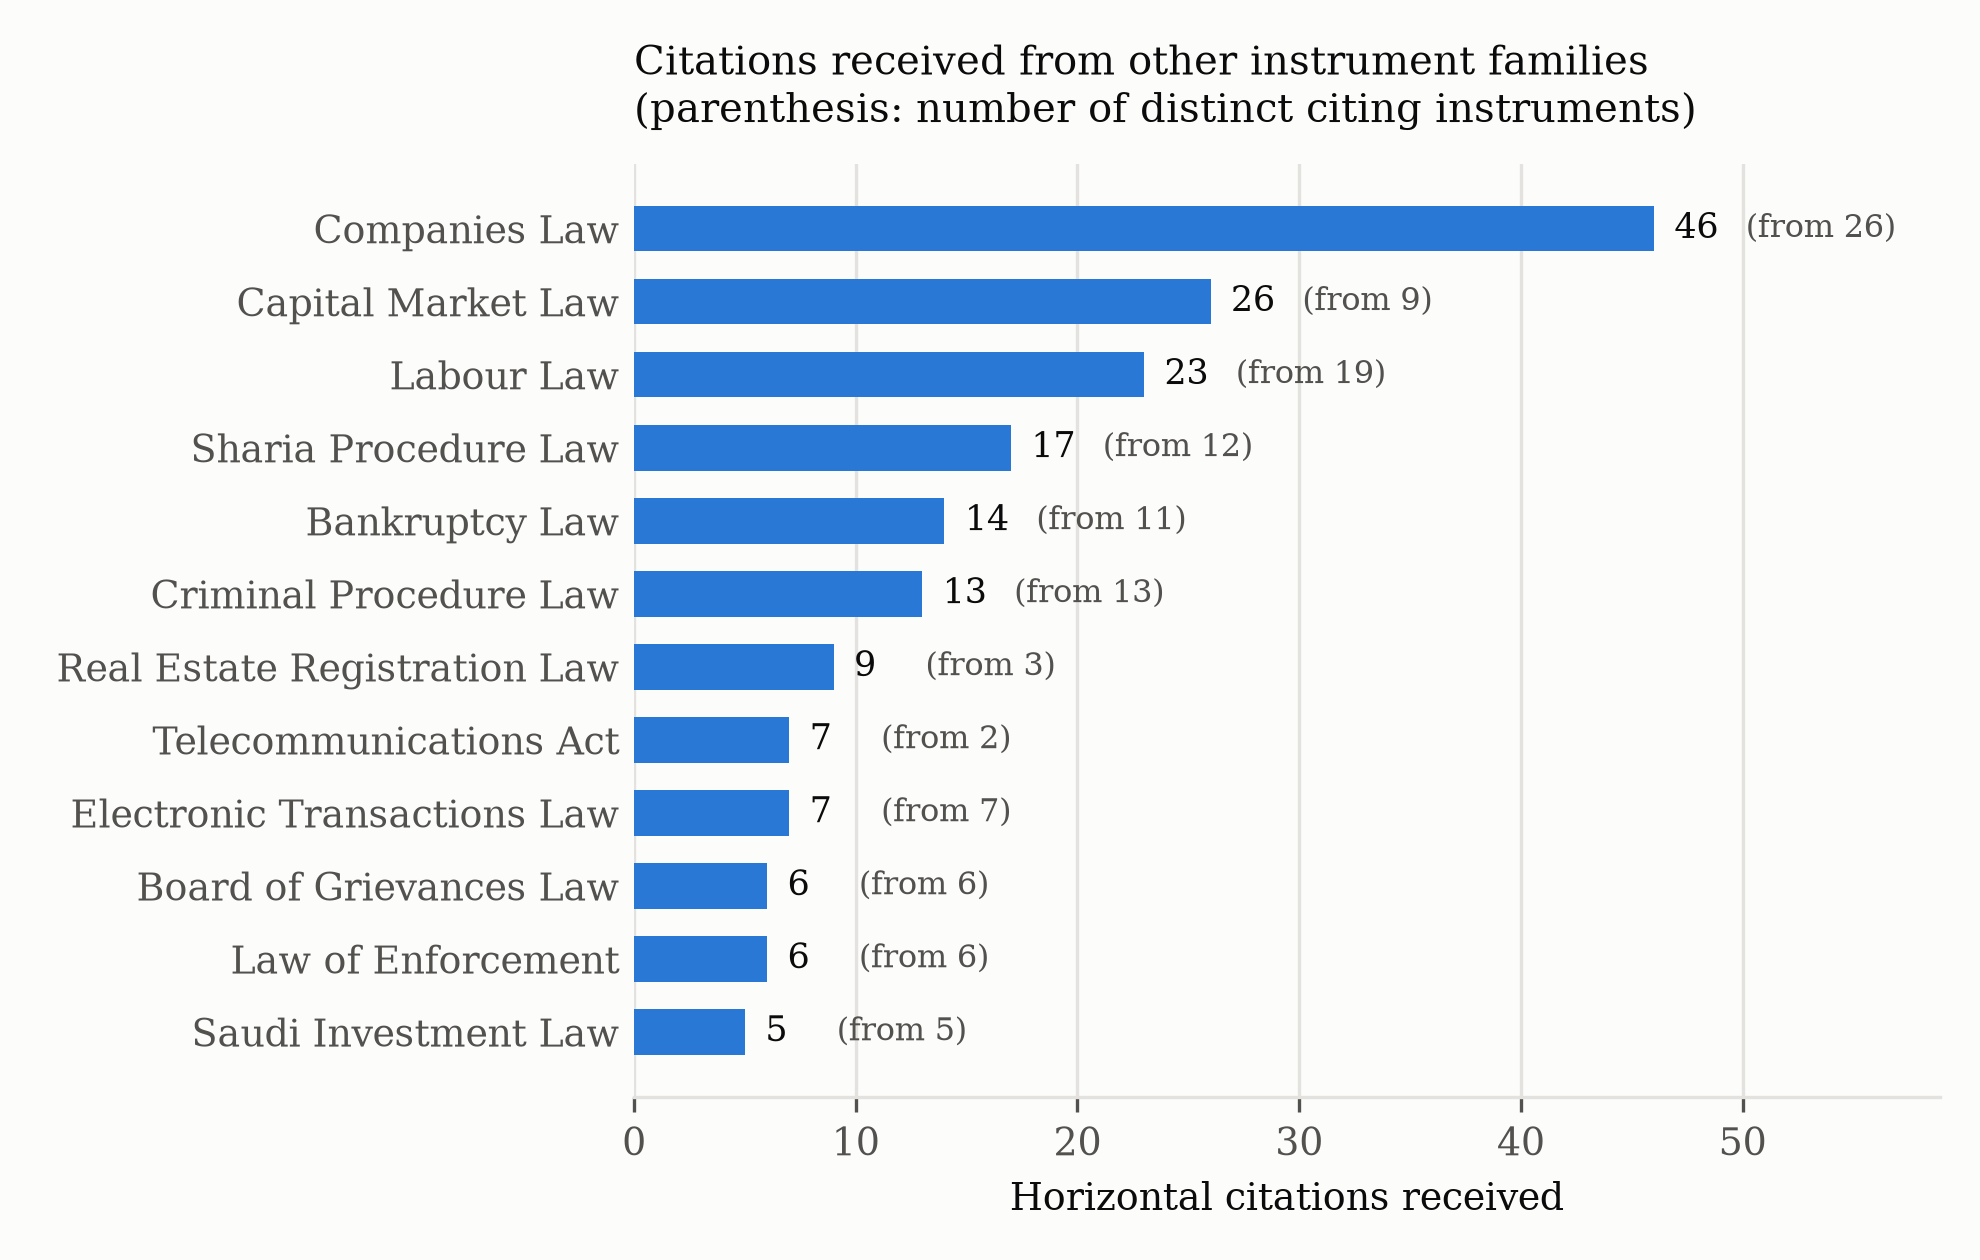
\includegraphics[width=\textwidth]{fig1_hubs.png}
\caption{Horizontal citations received by the twelve most-cited instruments.
The figure in parentheses is the number of \emph{distinct} instruments that
cite the target, which separates breadth from depth: the Capital Market Law
receives 26 citations but from only 9 instruments, while the Criminal
Procedure Law receives 13 citations from 13 distinct instruments.}
\label{fig:hubs}
\end{figure}

Figure~\ref{fig:hubs} shows the horizontal in-degree of the leading
instruments, with the number of distinct citing instruments alongside.

The \textbf{Companies Law} is the system's dominant hub: 46 horizontal
citations from 26 distinct instruments, nearly twice the count of any other
instrument and drawn from the widest range of sources. Its prominence is
intelligible --- nearly every economic regulation must settle who counts as a
company --- and it is robust to how family boundaries are drawn. The
\textbf{Labour Law} follows at 23 citations from 19 instruments, still the
second-broadest reach in the corpus but no longer a rival to the Companies
Law once its own annexes are excluded. That commercial and labour statutes
rather than, say, constitutional instruments occupy these positions tells us
something real about which parts of Saudi law are load-bearing in day-to-day
regulation.

Citation is heavily concentrated: the ten most-cited instruments receive
58.1\% of all horizontal citations, while 164 instruments participate in the
horizontal network at all. A small definitional core carries the system.

Breadth and depth come apart sharply. The \textbf{Capital Market Law} ranks
second by citation count (26) but draws them from only nine instruments: it
is cited intensively within the financial regulatory cluster and barely
outside it. By contrast the \textbf{Criminal Procedure Law} receives 13
citations from 13 distinct instruments, and the \textbf{Electronic
Transactions Law} 7 from 7 --- perfectly dispersed citation, the signature
of an instrument that supplies a general mechanism (here, the legal status
of electronic records) that many unrelated regimes need exactly once. A
ranking by raw count would treat the Capital Market Law as more central than
either; a ranking by breadth would reverse it. Both readings are legitimate
and they answer different questions, which is precisely why the two figures
should be reported together.

Weighted PageRank over the validated network puts the Companies Law first
(0.075), the Capital Market Law second (0.066), the Labour Law third
(0.047), and the Bankruptcy Law fourth (0.036). PageRank rewards the Capital
Market Law for being cited by instruments that are themselves cited, which
is consistent with its position at the centre of a dense financial cluster.

As a robustness check we recomputed the horizontal share and the leading
hubs on all 424 resolved edges, that is without dropping the 14
misresolutions. The horizontal share moves only from 70.5\% to 71.5\% and
the four leading hubs are unchanged, so the headline structural findings do
not depend on the validation step. The step still matters for individual
rankings further down the distribution, where instruments separated by one
or two citations change places --- which is precisely where a reader
interested in a specific instrument would look.

\subsection{Domain structure}

\begin{figure}[t]
\centering
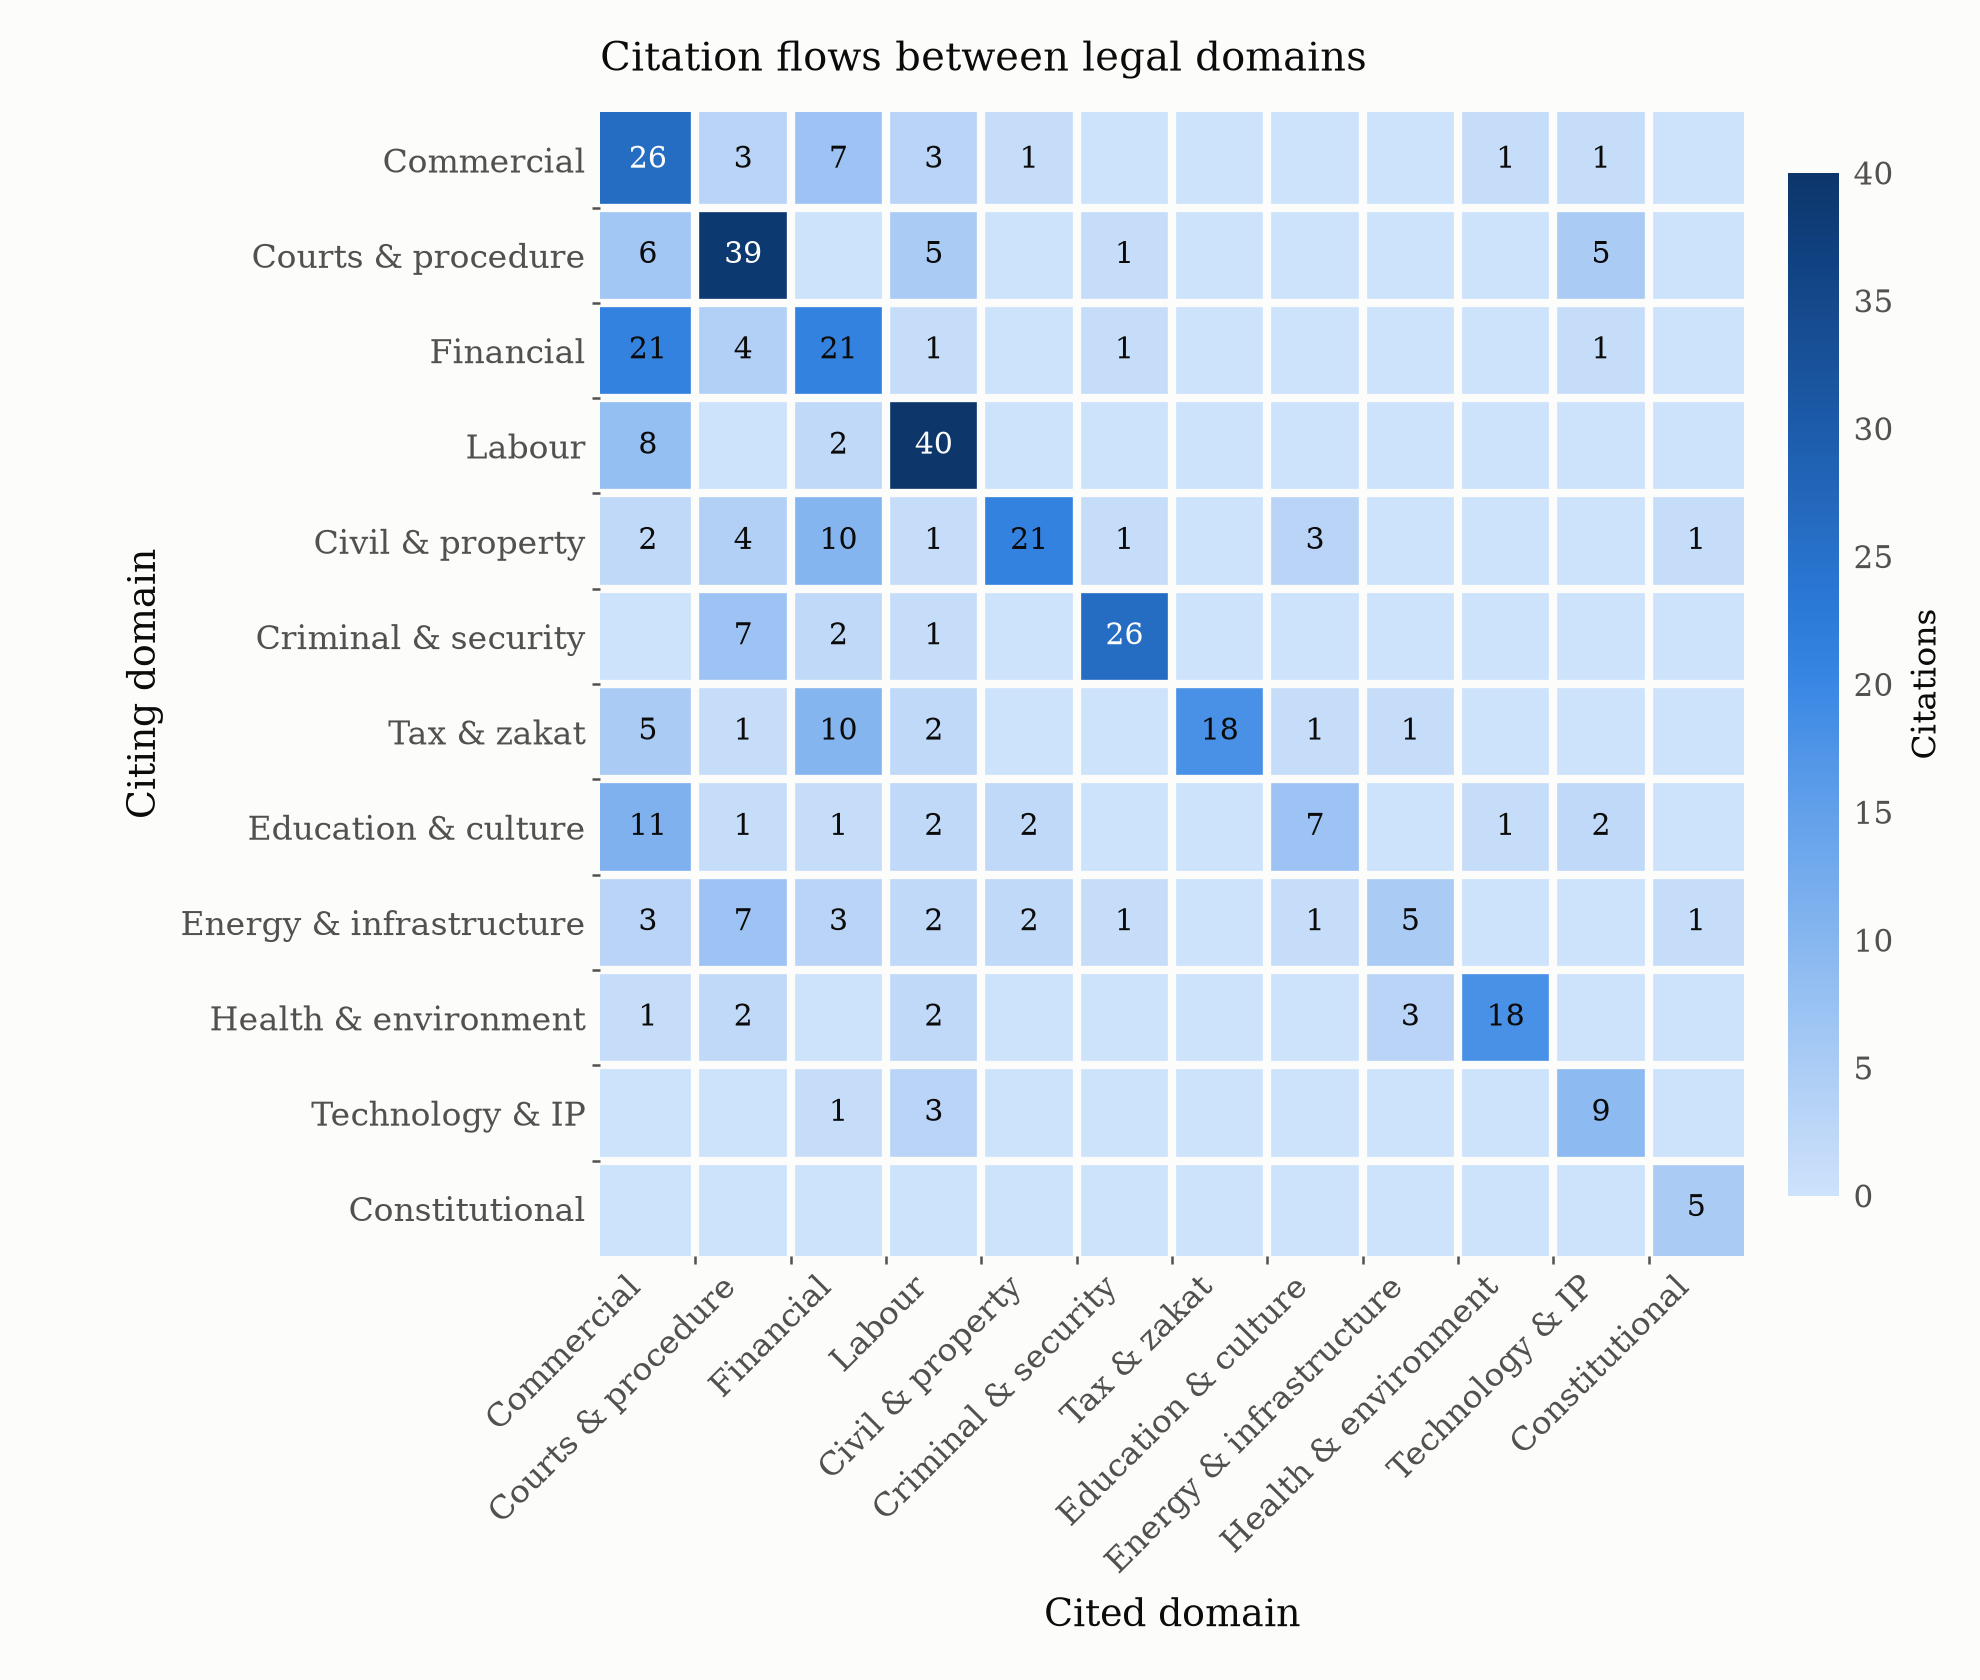
\includegraphics[width=\textwidth]{fig2_domain_flows.png}
\caption{Citation flows between legal domains. The diagonal carries
intra-domain citation; off-diagonal cells show which bodies of law reach
into which others. Domains follow the author-assigned grouping released with
the corpus.}
\label{fig:domains}
\end{figure}

Aggregating citations to the domain level (Figure~\ref{fig:domains}), 235 of
410 citations stay within a domain and 175 cross domains. The diagonal
dominates, as expected, but the off-diagonal structure is informative.

The heaviest cross-domain flow runs from \textbf{financial and capital
markets into commercial and corporate law} (21 citations) --- financial
regulation resting on company-law foundations. Tax and zakat instruments
cite financial ones (10); civil and property instruments cite financial ones
(10); education, culture and civil-society instruments cite commercial law
(11), reflecting that associations, cooperatives, and professional bodies
are constituted through commercial-law machinery. Courts and procedure sends
citations outward (to commercial law, 6; to technology and IP, 5) more than
it receives from most domains, which is what one expects of procedural law:
it is invoked by substantive regimes rather than invoking them.

The constitutional and administrative domain is almost entirely disconnected
from the rest of the citation network. This is not evidence that
constitutional instruments are unimportant; it reflects that foundational
instruments are presupposed rather than cited, a pattern also observed in
statutory networks elsewhere.

\subsection{Dangling citations to repealed instruments}
\label{sec:dangling}

The corpus ships a supersession graph of 102 repeal and replacement
relationships, each classified by hand from the instruments' own documented
text. Cross-referencing it against citations whose target the extractor
could \emph{not} resolve --- on the hypothesis that an unresolvable cited
name may be a repealed instrument no longer in force --- identifies
citations that point at law that has been superseded.

Matching is deliberately conservative. A cited name matches a repealed
instrument only when all of its content tokens appear in that instrument's
recorded description and it carries at least two such tokens. The
two-token floor is essential: single generic tokens such as
\emph{al-hay'ah} (``the Authority'') or \emph{al-'amal} (``work'') are
contained in many descriptions and generate false matches. Applying it
reduces an initial seven candidates to \textbf{three confirmed cases}:

\begin{itemize}
  \item The \emph{Implementing Regulation for Environmental Inspection and
    Audit} (Article~8) and the \emph{Implementing Regulation for
    Environmental Service Providers} (Article~12) both direct the reader to
    the implementing regulation on recording environmental violations and
    imposing penalties --- in the version that has since been replaced.
  \item The \emph{Foreigners' Residency Law} (Article~56) provides for
    prosecution under the General Civil Servants Law
    (\emph{ni\d{z}\={a}m al-muwa\d{z}\d{z}af\={\i}n al-'\={a}mm}), an
    instrument repealed in full by the Civil Service Law.
\end{itemize}

Three cases in a corpus of this size is a small number, and we resist
inflating it: the true figure is bounded below by our method, since we can
only detect repeals that the supersession graph records and citations whose
names are distinctive enough to match. What the finding demonstrates is that
the defect class \emph{exists} and is now \emph{detectable at scale}. In a
jurisdiction without a machine-readable consolidated gazette, a citation
pointing at repealed law is discoverable only by a reader who happens to
know the repeal --- or, from now on, by intersecting two released graphs.

\subsection{What Saudi legislation cites but no corpus contains}
\label{sec:absent}

The 161 references the extractor could not resolve are not merely
extraction noise. They name \textbf{128 distinct} instruments and provisions
that Saudi legislation actively relies on and that the corpus --- the most
comprehensive machine-readable collection of Saudi law available --- does not
contain. Some are older instruments superseded but still cited
(Section~\ref{sec:dangling}); others are live instruments not yet
consolidated in machine-readable form, among them retirement and pension
regimes, social-care regulations, and internal committee rules; and a
residue are formulaic references to instruments issued by decision of an
authority, which name no specific instrument at all.

Read as a coverage map, this set is a prioritised work list for anyone
extending machine-readable coverage of Saudi law: it identifies exactly
which absent instruments the existing corpus most often needs.

\section{Discussion}
\label{sec:discussion}

\paragraph{For legal informatics.}
The vertical/horizontal distinction generalises beyond Saudi Arabia. Any
jurisdiction that pairs statutes with implementing regulations will produce
citation networks in which hierarchical elaboration and systemic integration
are mixed, and any centrality ranking computed over the mixture will
overstate the importance of statutes that happen to carry long regulations.
Reporting the split costs little and changes conclusions.

\paragraph{For retrieval-augmented legal AI.}
Systems that answer questions about Saudi law by retrieving statutory text
inherit the structure measured here. Two implications follow. Retrieval that
returns a single article will frequently be insufficient, because the
governing rule lives in another instrument that the retrieved article cites
--- most often the Companies Law or the Labour Law, which between them
receive 69 horizontal citations from 45 distinct instruments. And a system that grounds answers in
statutory text without checking supersession can reproduce dangling
citations of exactly the kind identified in Section~\ref{sec:dangling},
faithfully quoting a provision that points at repealed law.

\paragraph{For legislative maintenance.}
The graphs released with this analysis make two maintenance questions
computable: which live instruments cite superseded law, and which cited
instruments lack a consolidated machine-readable text. Neither is answerable
by reading, at this scale, by anyone.

\section{Limitations}
\label{sec:limitations}

\paragraph{We measure the extractor's output, not the true citation network.}
The 585 inter-instrument references are those a deterministic pattern-based
extractor detected. Its recall is unmeasured: citations phrased in ways the
patterns do not cover are invisible to this study, and the resulting network
is therefore a lower bound on the system's true connectivity. Precision, by
contrast, we do measure, and correct, for the resolution step
(Section~\ref{sec:validation}).

\paragraph{Coverage bounds the network.}
The corpus covers 290 instruments, not every Saudi legislative instrument.
Citations to absent instruments become unresolved edges rather than network
structure, so measured centrality is centrality \emph{within the corpus}.

\paragraph{Dangling-citation detection is conservative.}
It depends on the supersession graph, which is hand-classified and
deliberately incomplete, and on name matching, which we constrained to avoid
false positives at the cost of recall. Three confirmed cases is a floor, not
an estimate.

\paragraph{Family assignment is heuristic.}
Vertical and horizontal citation are separated using the corpus's
subject-matter grouping, which is a good but imperfect proxy for legal
subordination. A subordinate instrument issued under a differently named
parent --- a capital-market authority regulation issued under the Capital
Market Law, for instance --- is counted as horizontal. The two readings we
report bound the effect of the ambiguity we could detect; they do not bound
this one, which would require explicit parent-instrument metadata that no
current source provides.

\paragraph{Hub interpretation is bounded by coverage and by counting.}
Instruments outside the corpus cannot accumulate citations, and citation
counts measure how often an instrument is invoked, not how consequential
each invocation is: a single reference that imports an entire licensing
regime counts the same as a passing definitional cross-reference. Centrality
here is a measure of referential load, not of legal importance.

\paragraph{The domain grouping is author-assigned.}
Domain membership is not a property of Saudi legislation; the twelve-domain
grouping used in Figure~\ref{fig:domains} is applied by published rules and
is an organising device, not a legal taxonomy.

\paragraph{The network is a snapshot.}
All instruments are analysed as of the corpus release. Because the corpus
records publication dates, the temporal analysis that
\citet{coupette2021measuring} perform for other jurisdictions is possible in
principle, and we leave it to future work.

\section{Conclusion}
\label{sec:conclusion}

We have constructed and analysed what is, to our knowledge, the first
citation network over Saudi
Arabian legislation: 290 instruments, 410 validated inter-instrument
citations, and a 3.3\% resolution-error rate measured rather than assumed.
The network is 70.5--74.4\% horizontal, sparse, overwhelmingly asymmetric,
and concentrated in a single component of 175 instruments centred on the
Companies Law, with the ten most-cited instruments absorbing 58\% of
horizontal citation. Separating vertical from horizontal citation was not a
refinement but a correction: under a naive family definition the Labour Law
appears to co-lead the system, and it does not. Separating breadth from
depth then reveals two further kinds of importance --- the intensively cited
Capital Market Law against the widely cited Criminal Procedure and
Electronic Transactions Laws --- that a raw citation count merges. Intersecting the citation network with
a supersession graph makes a previously invisible defect class detectable:
live instruments that cite repealed law.

The wider point is that this analysis became possible the moment a
provenance-annotated statutory corpus existed. The same is true of every
jurisdiction currently absent from the legal-network literature, which is to
say most of them.

\section*{Declarations}

\paragraph{Funding.} No funding was received for conducting this study.

\paragraph{Competing interests.} The author declares no competing interests.

\paragraph{Ethics approval.} Not applicable. The study involves no human
participants, no animal subjects, and no personal data; it analyses
published national legislation only.

\paragraph{Data availability.} The corpus, the citation and supersession
graphs, and the analysis and figure scripts that reproduce every number and
figure reported here are openly available at
\url{https://github.com/Abdullah-m7/saudi-legal-corpus-ai} and archived on
Zenodo under the MIT licence
(\href{https://doi.org/10.5281/zenodo.22019183}{10.5281/zenodo.22019183};
concept DOI
\href{https://doi.org/10.5281/zenodo.22019182}{10.5281/zenodo.22019182}).

\paragraph{Code availability.} All analysis code is included in the archived
release cited above.

\paragraph{Author contributions.} A.~Almohammedi is the sole author and
conducted all aspects of the work.

\paragraph{Legal status.} This paper analyses a non-official research corpus.
The corpus is not an official government publication, contains no official
translation, and nothing here constitutes legal advice; the binding text of
any instrument is the Arabic original published in \emph{Umm Al-Qura}.

\bibliographystyle{plainnat}
\bibliography{references}

\end{document}
